\documentclass[11pt,letterpaper]{article}
%\documentclass[11pt,letterpaper]{exam}
\usepackage[latin1]{inputenc}
\usepackage[left=3.00cm, right=3.00cm, top=3.00cm, bottom=3.00cm]{geometry}

\usepackage{amsmath}
%\usepackage{amsthm}
%\usepackage{cancel}
\usepackage{mathtools}
%\DeclarePairedDelimiter\ceil{\lceil}{\rceil}
%\DeclarePairedDelimiter\floor{\lfloor}{\rfloor}

\usepackage{fancyhdr}
\pagestyle{fancy}

\usepackage{color}
%\usepackage{xcolor}
%\usepackage{graphicx}
\usepackage{caption}
%\definecolor{acolour}{rgb}{0,0.0,0}

%\usepackage{url}
\usepackage{listings}
%\usepackage[]{algorithm2e}

\lstset{frame=tb,
	language=Java,
	aboveskip=3mm,
	belowskip=3mm,
	showstringspaces=false,
	%frame=tb,
	columns=flexible,
	basicstyle={\small\ttfamily},
	numbers=none,
	numberstyle=\tiny\color{gray},
	keywordstyle=\color{blue},
	commentstyle=\color{dkgreen},
	stringstyle=\color{mauve},
	breaklines=true,
	breakatwhitespace=true,
	tabsize=3
}

\newcounter{nalg}[section] % defines algorithm counter for chapter-level
\renewcommand{\thenalg}{\thechapter .\arabic{nalg}} %defines appearance of the algorithm counter
\DeclareCaptionLabelFormat{algocaption}{Algorithm \thenalg} % defines a new caption label as Algorithm x.y

\lstnewenvironment{algorithm}[1][] %defines the algorithm listing environment
{   
    \refstepcounter{nalg} %increments algorithm number
    \captionsetup{labelformat=algocaption,labelsep=colon} %defines the caption setup for: it uses label format as the declared caption label above and makes label and caption text to be separated by a ':'
    \lstset{ %this is the stype
        mathescape=true,
        frame=tB,
        numbers=left, 
        numberstyle=\tiny,
        basicstyle=\scriptsize, 
        keywordstyle=\color{blue}\bfseries\em,
        keywords={,input, output, return, datatype, function, in, if, else, foreach, while, begin, end, true, false, int, for, then, } %add the keywords you want, or load a language as Rubens explains in his comment above.
        numbers=left,
        xleftmargin=.02\textwidth,
        #1 % this is to add specific settings to an usage of this environment (for instnce, the caption and referable label)
    }
}
{}

\author{Simon Zheng\\260744353}
\title{Homework 4}
\date{November 18$^{\textnormal{th}}$, 2017}
\lhead{COMP 251}
%\chead{Homework $$}
\rhead{Algorithms and Data Structures}

\begin{document}
	\maketitle
	\thispagestyle{fancy}
	
	\section{Master Theorem}
		\begin{align*}
			\
		\end{align*}
	
	\section{Stock}
		Recursively divide the sequence in half until you only have sub-arrays of length 1 or 2.
		For each sub-array of length 2, find the difference.
		Keep track of a global maximal difference found (and the indices of the two values) and update it every time a difference is computed.
		
		Now merge back.
		At each merge, take the difference between
		
	\section{Huffman code tree}
		\begin{figure}[h]
			\centering
			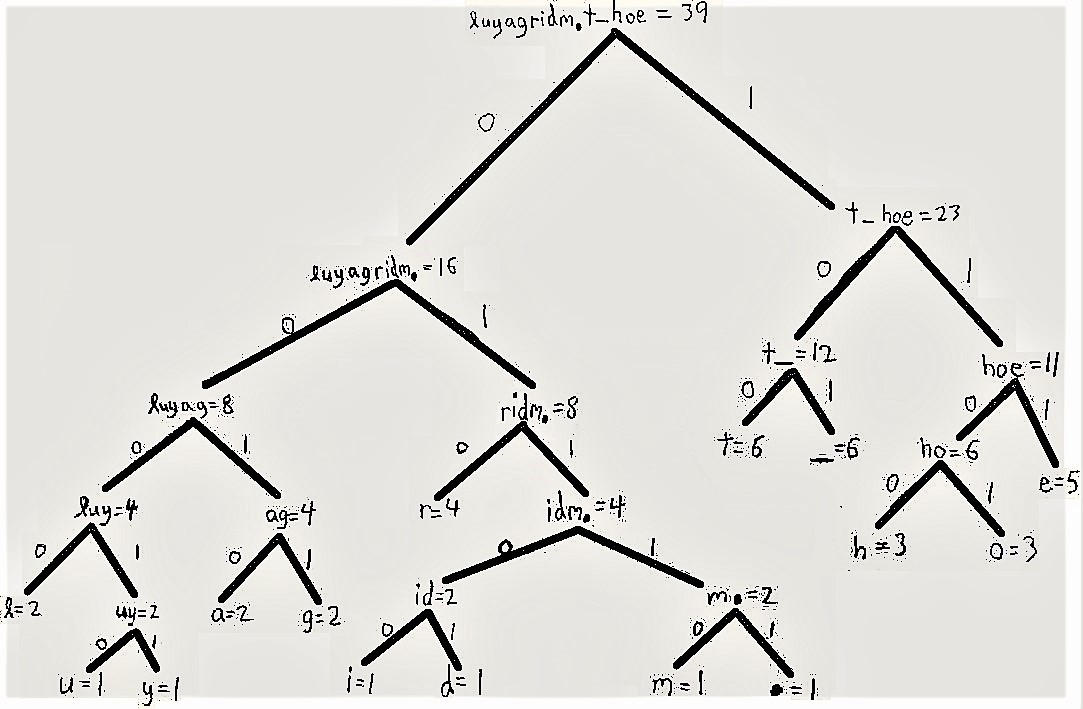
\includegraphics[width=360px,height=360px,keepaspectratio]{huffmancodetree.jpg}
			\linespread{0.8}\caption{Huffman code tree.}
		\end{figure}
		"that rug really tied the room together."
		\newline
		100 1100 0010 100 101 010 00010 0011 101 010 111 0010 0000 0000 00011 101 100 01100 111 01101 101 100 1100 111 101 010 1101 1101 01110 101 100 1101 0011 111 100 1100 111 010 01111
	
	\section{Compression scheme}
		By the pigeonhole principle.
		\newline
		\newline
		We have $256^n = 2^{8n}$ possible strings for an n-character file (ASCII is 8-bit which gives us 256 distinct characters).
		
		To be able to compress some files to smaller sizes yet still be an injective map, a single compression scheme must map other files into bigger sizes.
		Otherwise, we could infinitely compress a file by running the compression scheme's algorithm repeatedly.
		
		When compressing we want to be able to reliably decompress it (no loss of information) so we need a unique mapping for every distinct file (combination of string) which is why it must be injective (or at least bijective).
		
		In an $n$-byte file there are $8n$ bits to represent all 256 distinct characters in ASCII.
		As such, there are $2^n$ distinct possible files of $n$-characters where each character can be one of $2^8$ distinct characters.
		
		With a lossless compression (injective map), each permutation of character and each change of even a single character must map to a distinct encoding.
		
		We can already have an intuition of why there must exist a string (file) $x$ such that $C(x)$ gives an equal or greater size, if we mapped other files/strings to distinct smaller one.
		
		We compress $2^{8n}$ bits into a smaller size (less bits).
		But, as explained previously, there also has to be $2^{8n}$ possible mappings to distinguish between them, so the set of inputs has the same size as the set of outputs.
		
		But a compression scheme tries to map the set of all inputs into a smaller set of outputs since, if it compresses, with less bits, there are less possible distinct elements.
		Therefore, we get a surjection and some strings will get mapped to the same output, thus we get collisions.
		
		The only way around this, is if we let certain strings be mapped to the same length or longer, since we need extra bits for when we run out of the smaller number off bits which were already mapped onto by compressed files.
		\newline
		\newline
		So, to recap:
		\newline
		\newline
		We need $2^{8n}$ bits to represent $n$ distinct characters in binary.
		But these characters can be arranged into $2^{8n}$ distinct ways.
		The best $C$ can do is getting down to $2^n$ bits (after all, we still have to keep the $n$ characters somehow).
		
		But this means only $2^{8n} - 2^n$ distinct possible files are covered.
		For the rest, we need more bits to represent them distinctly.
		Thus, by the pigeonhole principle, there must be \textit{some} $x$ in $\Omega^n$ such that $\left|C(x)\right| \geq 8n$.
		
	\section{Tile board}
		Keep recursively dividing the board into 4 smaller and smaller "quadrants" (as it is of size $2^n \times 2^n$) until you get to single tiles.
		
		We will start from the missing cell (a single tile).
		
		First, "merge" back up one level so you get $2 \times 2$ quadrants.
		If a quadrant contains the empty cell, then there must be 3 empty cells in an L shape, so put a tile on it.
		
		Now, together with the 3 other quadrants (that will form a bigger quadrant in the "upper" recursion level), put a tile in the center of all 4.
		Since the quadrant containing the empty cell is filled, the center 4 cells will have one filled cell, and the 3 others will be empty and in an L shape, just like previously, so fill them with a tile.
		
		Doing this means that the 3 other quadrants (that didn't contain the empty cell) are going to have one cell filled, and will each have 3 empty cells left in an L shape, so fill them with tiles.
		
		Keep doing this recursively, where in every recursion layer you always start by filling the center 4 cells with a tile, as there will be a single cell filled previously in a lower recursion level.
		
		We can use a double array matrix and separate them by index ranges (e.g. for $0 \leq i,j \le 4$, etc.) and start from the already filled sub-board (the empty cell in the base case) and then fill the quadrants clockwise (after putting the center tile).\newline
		\linebreak This works by induction.
		If $2^n \times 2^n$ is the dimension of the board:
		
		Base case $P(n)=P(1)$: We have a $2 \times 2$ square board. Remove any of the cells. You will be left with 3 cells in an L shape.
		
		Induction hypothesis: For any $2^n \times 2^n$ square board with a single missing cell, you can fill it with L-shaped 3-cell tiles.
		
		Induction step $P(n+1)$: If the previous board P(n) is part of a bigger $2^n \times 2^n$ board, then it must be with 3 other same size board in a quadrant fashion (to form a square). We know that they are all empty except for the "sub-board" we previously filled. Therefore, at the center of the "super-board", there must be 4 cells which are the corners of each sub-board that touches each other, with one that filled or has the missing cell. We can put a tile on the 3 others, and as such the 3 other sub-board will each have a single cell filled. Thus, to fill the 3 other boards, we do the same thing as the first as it is the same case, just that the newly filled cells act like the missing cell in the first sub-board.
		
		As for the running time, if $n$ is the number of cells, which is a power of 4, then
	
	\section{Triple cycles}
		Make an adjacency matrix of the outgoing edges.
		
		We can think of marking adjacent vertices with a 1 as saying there is a path of length 1 between them.
		
		We also know that matrix multiplication of two $n \times n$ matrices, where $i$ is a row and $j$ is a column, each $i,j$-th entry of the resulting matrix is:
		$\sum_{k=1}^{n}A_{ik}B_{kj}$
		where we sum the entries over $k$ every time.
		
		So multiplying an adjacency matrix by itself $n$ times is the equivalent of finding all the paths of length $n$ as if a path "stops" it becomes 0, but if it continues it will get added (the path to the next vertex).
		
		So what we want is to cube it to get paths of length 3, which is $o(n^3)$.
		The diagonal is where paths came back to the original vertex of that column/row, as it contains the entries corresponding to the paths of each of the vertices to themselves, so just sum it (get the trace) to get all triple cycles.
		
		If $a \rightarrow b \rightarrow c \rightarrow a$ and $b \rightarrow c \rightarrow a \rightarrow b$ are considered the same triple (also same for when starting at $c$), then divide the trace by 3.
	
\end{document}
